\documentclass[]{book}
\usepackage{lmodern}
\usepackage{amssymb,amsmath}
\usepackage{ifxetex,ifluatex}
\usepackage{fixltx2e} % provides \textsubscript
\ifnum 0\ifxetex 1\fi\ifluatex 1\fi=0 % if pdftex
  \usepackage[T1]{fontenc}
  \usepackage[utf8]{inputenc}
\else % if luatex or xelatex
  \ifxetex
    \usepackage{mathspec}
  \else
    \usepackage{fontspec}
  \fi
  \defaultfontfeatures{Ligatures=TeX,Scale=MatchLowercase}
\fi
% use upquote if available, for straight quotes in verbatim environments
\IfFileExists{upquote.sty}{\usepackage{upquote}}{}
% use microtype if available
\IfFileExists{microtype.sty}{%
\usepackage{microtype}
\UseMicrotypeSet[protrusion]{basicmath} % disable protrusion for tt fonts
}{}
\usepackage{hyperref}
\hypersetup{unicode=true,
            pdftitle={Seminário Latinoamericano: Instrumentos y metodologias para un observatório de Clima y su impacto en la salud humana},
            pdfauthor={Sergio Ibarra-Espinosa},
            pdfborder={0 0 0},
            breaklinks=true}
\urlstyle{same}  % don't use monospace font for urls
\usepackage{natbib}
\bibliographystyle{apalike}
\usepackage{color}
\usepackage{fancyvrb}
\newcommand{\VerbBar}{|}
\newcommand{\VERB}{\Verb[commandchars=\\\{\}]}
\DefineVerbatimEnvironment{Highlighting}{Verbatim}{commandchars=\\\{\}}
% Add ',fontsize=\small' for more characters per line
\usepackage{framed}
\definecolor{shadecolor}{RGB}{248,248,248}
\newenvironment{Shaded}{\begin{snugshade}}{\end{snugshade}}
\newcommand{\AlertTok}[1]{\textcolor[rgb]{0.94,0.16,0.16}{#1}}
\newcommand{\AnnotationTok}[1]{\textcolor[rgb]{0.56,0.35,0.01}{\textbf{\textit{#1}}}}
\newcommand{\AttributeTok}[1]{\textcolor[rgb]{0.77,0.63,0.00}{#1}}
\newcommand{\BaseNTok}[1]{\textcolor[rgb]{0.00,0.00,0.81}{#1}}
\newcommand{\BuiltInTok}[1]{#1}
\newcommand{\CharTok}[1]{\textcolor[rgb]{0.31,0.60,0.02}{#1}}
\newcommand{\CommentTok}[1]{\textcolor[rgb]{0.56,0.35,0.01}{\textit{#1}}}
\newcommand{\CommentVarTok}[1]{\textcolor[rgb]{0.56,0.35,0.01}{\textbf{\textit{#1}}}}
\newcommand{\ConstantTok}[1]{\textcolor[rgb]{0.00,0.00,0.00}{#1}}
\newcommand{\ControlFlowTok}[1]{\textcolor[rgb]{0.13,0.29,0.53}{\textbf{#1}}}
\newcommand{\DataTypeTok}[1]{\textcolor[rgb]{0.13,0.29,0.53}{#1}}
\newcommand{\DecValTok}[1]{\textcolor[rgb]{0.00,0.00,0.81}{#1}}
\newcommand{\DocumentationTok}[1]{\textcolor[rgb]{0.56,0.35,0.01}{\textbf{\textit{#1}}}}
\newcommand{\ErrorTok}[1]{\textcolor[rgb]{0.64,0.00,0.00}{\textbf{#1}}}
\newcommand{\ExtensionTok}[1]{#1}
\newcommand{\FloatTok}[1]{\textcolor[rgb]{0.00,0.00,0.81}{#1}}
\newcommand{\FunctionTok}[1]{\textcolor[rgb]{0.00,0.00,0.00}{#1}}
\newcommand{\ImportTok}[1]{#1}
\newcommand{\InformationTok}[1]{\textcolor[rgb]{0.56,0.35,0.01}{\textbf{\textit{#1}}}}
\newcommand{\KeywordTok}[1]{\textcolor[rgb]{0.13,0.29,0.53}{\textbf{#1}}}
\newcommand{\NormalTok}[1]{#1}
\newcommand{\OperatorTok}[1]{\textcolor[rgb]{0.81,0.36,0.00}{\textbf{#1}}}
\newcommand{\OtherTok}[1]{\textcolor[rgb]{0.56,0.35,0.01}{#1}}
\newcommand{\PreprocessorTok}[1]{\textcolor[rgb]{0.56,0.35,0.01}{\textit{#1}}}
\newcommand{\RegionMarkerTok}[1]{#1}
\newcommand{\SpecialCharTok}[1]{\textcolor[rgb]{0.00,0.00,0.00}{#1}}
\newcommand{\SpecialStringTok}[1]{\textcolor[rgb]{0.31,0.60,0.02}{#1}}
\newcommand{\StringTok}[1]{\textcolor[rgb]{0.31,0.60,0.02}{#1}}
\newcommand{\VariableTok}[1]{\textcolor[rgb]{0.00,0.00,0.00}{#1}}
\newcommand{\VerbatimStringTok}[1]{\textcolor[rgb]{0.31,0.60,0.02}{#1}}
\newcommand{\WarningTok}[1]{\textcolor[rgb]{0.56,0.35,0.01}{\textbf{\textit{#1}}}}
\usepackage{longtable,booktabs}
\usepackage{graphicx,grffile}
\makeatletter
\def\maxwidth{\ifdim\Gin@nat@width>\linewidth\linewidth\else\Gin@nat@width\fi}
\def\maxheight{\ifdim\Gin@nat@height>\textheight\textheight\else\Gin@nat@height\fi}
\makeatother
% Scale images if necessary, so that they will not overflow the page
% margins by default, and it is still possible to overwrite the defaults
% using explicit options in \includegraphics[width, height, ...]{}
\setkeys{Gin}{width=\maxwidth,height=\maxheight,keepaspectratio}
\IfFileExists{parskip.sty}{%
\usepackage{parskip}
}{% else
\setlength{\parindent}{0pt}
\setlength{\parskip}{6pt plus 2pt minus 1pt}
}
\setlength{\emergencystretch}{3em}  % prevent overfull lines
\providecommand{\tightlist}{%
  \setlength{\itemsep}{0pt}\setlength{\parskip}{0pt}}
\setcounter{secnumdepth}{5}
% Redefines (sub)paragraphs to behave more like sections
\ifx\paragraph\undefined\else
\let\oldparagraph\paragraph
\renewcommand{\paragraph}[1]{\oldparagraph{#1}\mbox{}}
\fi
\ifx\subparagraph\undefined\else
\let\oldsubparagraph\subparagraph
\renewcommand{\subparagraph}[1]{\oldsubparagraph{#1}\mbox{}}
\fi

%%% Use protect on footnotes to avoid problems with footnotes in titles
\let\rmarkdownfootnote\footnote%
\def\footnote{\protect\rmarkdownfootnote}

%%% Change title format to be more compact
\usepackage{titling}

% Create subtitle command for use in maketitle
\providecommand{\subtitle}[1]{
  \posttitle{
    \begin{center}\large#1\end{center}
    }
}

\setlength{\droptitle}{-2em}

  \title{Seminário Latinoamericano: Instrumentos y metodologias para un observatório de Clima y su impacto en la salud humana}
    \pretitle{\vspace{\droptitle}\centering\huge}
  \posttitle{\par}
    \author{Sergio Ibarra-Espinosa}
    \preauthor{\centering\large\emph}
  \postauthor{\par}
      \predate{\centering\large\emph}
  \postdate{\par}
    \date{2019-09-08}

\usepackage{booktabs}
\usepackage{amsthm}
\makeatletter
\def\thm@space@setup{%
  \thm@preskip=8pt plus 2pt minus 4pt
  \thm@postskip=\thm@preskip
}
\makeatother

\begin{document}
\maketitle

{
\setcounter{tocdepth}{1}
\tableofcontents
}
\hypertarget{curso-de-r-contaminacion-atmosferica-y-mas}{%
\chapter*{Curso de R, contaminacion atmosferica y mas}\label{curso-de-r-contaminacion-atmosferica-y-mas}}
\addcontentsline{toc}{chapter}{Curso de R, contaminacion atmosferica y mas}

Este curso online contendra las sisgueinetes informaciones

\begin{itemize}
\tightlist
\item
  Sistemas de informacion con dartos de salud en Chile (gracias Paty Matus)
\item
  Impacto de las emisiones antropogenicas en la salud y clima
\item
  R desde Excel
\item
  Leer y procesar vectores espaciales con \textbf{sf} \citep{sf}
\item
  Leer y procesar informacion en grillas espaciales (raster) con stars\citep{stars} y raster\citep{raster}
\end{itemize}

\hypertarget{aprender-git}{%
\section*{Aprender Git}\label{aprender-git}}
\addcontentsline{toc}{section}{Aprender Git}

Para aprender GIT puedes ver:

\begin{itemize}
\tightlist
\item
  \url{https://git-scm.com/book/es/v1/Empezando}
\item
  \url{https://learngitbranching.js.org/}
\item
  \url{https://try.github.io/}
\end{itemize}

\hypertarget{clonar-este-contenido}{%
\section*{Clonar este contenido}\label{clonar-este-contenido}}
\addcontentsline{toc}{section}{Clonar este contenido}

Para clonar este contenido haz:

\begin{Shaded}
\begin{Highlighting}[]
\FunctionTok{git}\NormalTok{ clone https://github.com/ibarraespinosa/UBA.git}
\end{Highlighting}
\end{Shaded}

\hypertarget{intro}{%
\chapter{Sistemas de informacion con datos de salud en Chile}\label{intro}}

\begin{itemize}
\tightlist
\item
  Sistema de información en salud existentes
\item
  Enfasis en las fuentes de información y las escala temporal/espacial que manejan
\item
  Series de tiempo disponible por fuente
\item
  Instituciones a cargo de la captura, procesamiento y análisis
\item
  Disponibilidad de los datos e indicadores que producen
\item
  Otros
\end{itemize}

\hypertarget{encuesta-nacional-de-salud-ens}{%
\section{\texorpdfstring{\href{http://www.encuestas.uc.cl/ens/index.html}{Encuesta Nacional de Salud (ENS)}}{Encuesta Nacional de Salud (ENS)}}\label{encuesta-nacional-de-salud-ens}}

La ENS es una encuesta realizada por el Ministerio de Salud para identificar cuales son las
enfermedades que sufren y los tratamientos que reciben todas las personas con mas de 15 años
que viven en Chile. De esta forma es posible es posible realizar diagnosticos,
identificar problemas y formular politicas planes y proyectos para mejor la salud de las personas.

\begin{itemize}
\tightlist
\item
  \emph{Organismo responsable}: Ministerio de Salud, Departamento de Epidemiología\\
  Gobierno de Chile.\\
\item
  \emph{Organismo ejecutor}: Pontificia Universidad Católica de Chile (PUC).\\
\item
  \emph{Población objetivo}: Personas de 15 años y más, chilenas o extranjeras que residen habitualmente en viviendas particulares ocupadas, localizadas en zonas urbanas y rurales de las quince regiones de Chile.\\
\item
  \emph{Representatividad}: Nacional, regional y Urbano/Rural.\\
\item
  \emph{Modo de aplicación}: Entrevista personal en hogar (Sistema de captura electrónica: Tablet), aplicada por encuestador y profesional enfermera de acuerdo al tipo de cuestionario.\\
\item
  \emph{Período de trabajo de campo}: Agosto 2016 a marzo 2017\\
\item
  \emph{Tamaño muestral}: 6.233 encuestados, de los cuales 5.520 cuentan con exámenes de laboratorio de acuerdo a protocolo. 37,1\% hombres, 62,9\% mujeres.\\
\item
  \emph{Error muestral}: Error absoluto de muestreo de 2,6\% a nivel nacional, raíz del efecto de diseño de 1,797, estimaciones con 95\% de confianza y error relativo inferior a 30\%.
\end{itemize}

Algunos resultados:

\begin{itemize}
\tightlist
\item
  Consumo de tabaco: 66,7\% no fuma, 33,\$ fuma.
\item
  Consumo riesgoso de alcohol 11,7\%, 20,5\% hombres, 3,3\% mujeres.
\item
  Sedentarismo: 86,7\%, 83,3\% hombre, 90.0\% mujeres.
\item
  Estado nutricional: 1,3\% enfraquecido, 24,5\% normal, 39,8\% sobrepeso, 31,2\% obeso, 3,2\% obeso morbido.
\item
  Sospecha de hipertension: 27,6\%.
\item
  Sospecha de diabetes: 12,3\%.
\item
  Autoreporte de infarto agudo al miocardio: 3,3\%.
\item
  Autoreporte de ataque cerebro vascular: 2,6\%.
\end{itemize}

Fuentes:

\begin{itemize}
\tightlist
\item
  \url{https://www.minsal.cl/wp-content/uploads/2017/11/ENS-2016-17_PRIMEROS-RESULTADOS.pdf}
\item
  \url{https://www.minsal.cl/wp-content/uploads/2018/01/2-Resultados-ENS_MINSAL_31_01_2018.pdf}
\item
  \url{http://www.encuestas.uc.cl/ens/index.html}
\end{itemize}

\hypertarget{departamento-de-estadisticas-e-informaciones-de-salud}{%
\section{\texorpdfstring{\href{http://www.deis.cl/}{Departamento de Estadisticas e Informaciones de Salud}}{Departamento de Estadisticas e Informaciones de Salud}}\label{departamento-de-estadisticas-e-informaciones-de-salud}}

\begin{itemize}
\tightlist
\item
  Resúmenes estadísticos mensuales (\href{http://www.deis.cl/bases-de-datos-rem/}{REM}). Vea el \href{http://estadisticas.ssosorno.cl/estadisticas/2017/manuales/2017-2018-Manual-Series-REM-V1.1.pdf}{manual}
\item
  \href{http://www.deis.cl/bases-de-datos-defunciones/}{Defunciones}
\item
  \href{http://www.deis.cl/descargar-bases-de-datos-2/?page_id=3487}{Egresos}
\item
  \href{http://www.deis.cl/descargar-bases-de-datos-2/?page_id=3493}{Nacimientos}
\item
  \href{http://www.deis.cl/descargar-bases-de-datos-2/?page_id=3499}{Atenciones de urgencia}
\item
  \href{http://www.deis.cl/descargar-bases-de-datos-2/?page_id=3784}{Enfermedades de notificacion obligatoria}
\item
  \href{http://www.deis.cl/estadisticas-eta/}{Enfermedades transmitidas por alimentos}
\item
  \href{http://www.deis.cl/?page_id=3946}{Tuberculosis}
\end{itemize}

\hypertarget{encuesta-de-caracterizacion-socioeconomica-casen}{%
\section{\texorpdfstring{\href{http://observatorio.ministeriodesarrollosocial.gob.cl/casen-multidimensional/casen/casen_2017.php}{Encuesta de caracterizacion socioeconomica (CASEN)}}{Encuesta de caracterizacion socioeconomica (CASEN)}}\label{encuesta-de-caracterizacion-socioeconomica-casen}}

``La Encuesta de Caracterización Socioeconómica Nacional (Casen) del Ministerio de Desarrollo Social es una encuesta a hogares, de carácter multipropósito, es decir, que abarca diversos temas como educación, trabajo, ingresos, salud, entre otros; además es una encuesta transversal, por lo tanto, incluye a todo el espectro de la población del país.''

\hypertarget{estadisticas-generales}{%
\section{Estadisticas generales}\label{estadisticas-generales}}

\begin{itemize}
\tightlist
\item
  \href{www.ine.cl}{Instituto Nacional de Estadisticas}
\end{itemize}

\hypertarget{cepal-stat}{%
\section{CEPAL STAT}\label{cepal-stat}}

\begin{itemize}
\tightlist
\item
  \href{http://estadisticas.cepal.org/cepalstat/WEB_CEPALSTAT/estadisticasIndicadores.asp}{Estadisticos e indicadores}
\item
  \href{http://estadisticas.cepal.org/cepalstat/WEB_CEPALSTAT/estadisticasIndicadores.asp}{Perfiles Nacionales}
\item
  \href{http://estadisticas.cepal.org/cepalstat/WEB_CEPALSTAT/PublicacionesEstadisticas.asp}{Publicaciones y estadisticas}
\end{itemize}

\hypertarget{banco-interamericano-de-desarrollo}{%
\section{Banco Interamericano de Desarrollo}\label{banco-interamericano-de-desarrollo}}

\begin{itemize}
\tightlist
\item
  \href{http://www.iadb.org/en/research-and-data//tables,6882.html?indicator=2}{Educacion}
\item
  \href{http://www.iadb.org/en/research-and-data//tables,6882.html?indicator=2}{Mercado Laboral}
\item
  \href{http://www.iadb.org/es/investigacion-y-datos//tablas,6882.html?indicator=4}{Ingreso}
\item
  \href{http://www.iadb.org/es/investigacion-y-datos//pobreza,7526.html}{Pobreza}
\item
  \href{http://www.iadb.org/es/investigacion-y-datos//tablas,6882.html?indicator=1}{Demografia}
\end{itemize}

Egresos hospitalarios 2001 -- 2016

Natalidad 2011

Mortalidad 1994 -- 2016

Casen 2009-2016

You can label chapter and section titles using \texttt{\{\#label\}} after them, e.g., we can reference Chapter \ref{intro}. If you do not manually label them, there will be automatic labels anyway, e.g., Chapter \ref{methods}.

Figures and tables with captions will be placed in \texttt{figure} and \texttt{table} environments, respectively.

\begin{Shaded}
\begin{Highlighting}[]
\KeywordTok{par}\NormalTok{(}\DataTypeTok{mar =} \KeywordTok{c}\NormalTok{(}\DecValTok{4}\NormalTok{, }\DecValTok{4}\NormalTok{, }\FloatTok{.1}\NormalTok{, }\FloatTok{.1}\NormalTok{))}
\KeywordTok{plot}\NormalTok{(pressure, }\DataTypeTok{type =} \StringTok{'b'}\NormalTok{, }\DataTypeTok{pch =} \DecValTok{19}\NormalTok{)}
\end{Highlighting}
\end{Shaded}

\begin{figure}

{\centering 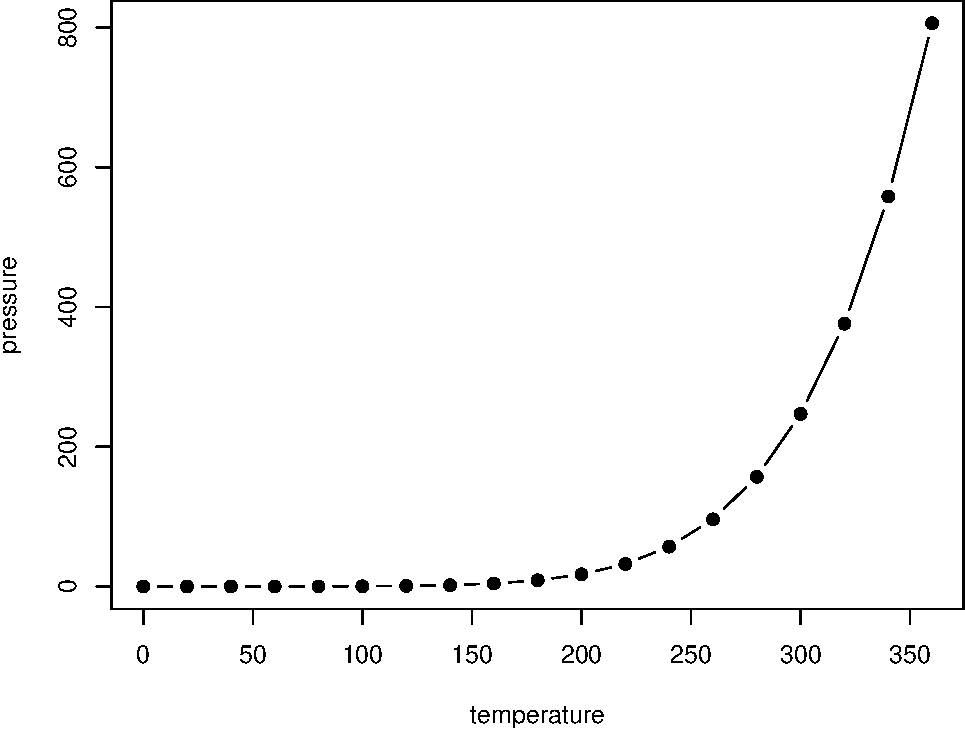
\includegraphics[width=0.8\linewidth]{bookdown-demo_files/figure-latex/nice-fig-1} 

}

\caption{Here is a nice figure!}\label{fig:nice-fig}
\end{figure}

Reference a figure by its code chunk label with the \texttt{fig:} prefix, e.g., see Figure \ref{fig:nice-fig}. Similarly, you can reference tables generated from \texttt{knitr::kable()}, e.g., see Table \ref{tab:nice-tab}.

\begin{Shaded}
\begin{Highlighting}[]
\NormalTok{knitr}\OperatorTok{::}\KeywordTok{kable}\NormalTok{(}
  \KeywordTok{head}\NormalTok{(iris, }\DecValTok{20}\NormalTok{), }\DataTypeTok{caption =} \StringTok{'Here is a nice table!'}\NormalTok{,}
  \DataTypeTok{booktabs =} \OtherTok{TRUE}
\NormalTok{)}
\end{Highlighting}
\end{Shaded}

\begin{table}[t]

\caption{\label{tab:nice-tab}Here is a nice table!}
\centering
\begin{tabular}{rrrrl}
\toprule
Sepal.Length & Sepal.Width & Petal.Length & Petal.Width & Species\\
\midrule
5.1 & 3.5 & 1.4 & 0.2 & setosa\\
4.9 & 3.0 & 1.4 & 0.2 & setosa\\
4.7 & 3.2 & 1.3 & 0.2 & setosa\\
4.6 & 3.1 & 1.5 & 0.2 & setosa\\
5.0 & 3.6 & 1.4 & 0.2 & setosa\\
\addlinespace
5.4 & 3.9 & 1.7 & 0.4 & setosa\\
4.6 & 3.4 & 1.4 & 0.3 & setosa\\
5.0 & 3.4 & 1.5 & 0.2 & setosa\\
4.4 & 2.9 & 1.4 & 0.2 & setosa\\
4.9 & 3.1 & 1.5 & 0.1 & setosa\\
\addlinespace
5.4 & 3.7 & 1.5 & 0.2 & setosa\\
4.8 & 3.4 & 1.6 & 0.2 & setosa\\
4.8 & 3.0 & 1.4 & 0.1 & setosa\\
4.3 & 3.0 & 1.1 & 0.1 & setosa\\
5.8 & 4.0 & 1.2 & 0.2 & setosa\\
\addlinespace
5.7 & 4.4 & 1.5 & 0.4 & setosa\\
5.4 & 3.9 & 1.3 & 0.4 & setosa\\
5.1 & 3.5 & 1.4 & 0.3 & setosa\\
5.7 & 3.8 & 1.7 & 0.3 & setosa\\
5.1 & 3.8 & 1.5 & 0.3 & setosa\\
\bottomrule
\end{tabular}
\end{table}

You can write citations, too. For example, we are using the \textbf{bookdown} package \citep{R-bookdown} in this sample book, which was built on top of R Markdown and \textbf{knitr} \citep{xie2015}.

\hypertarget{impacto-de-las-emisiones-antropogenicas-en-la-salud-y-clima}{%
\chapter{Impacto de las emisiones antropogenicas en la salud y clima}\label{impacto-de-las-emisiones-antropogenicas-en-la-salud-y-clima}}

\hypertarget{contaminacion-atmosferica}{%
\section{Contaminacion atmosferica}\label{contaminacion-atmosferica}}

La ciencia de la contaminacion atmosferica, si bien reciente, ha sido desarrollada debido a los avances de en la comprension
de la meteorologia.

Problemas relacionados con la contaminacion atmosferica han sido descritos en obras literarias y cartas a lo largo de
la historia. Por ejemplo, se cree que el primer caso reportado sobre los efectos de la contaminacion atmosférica en la salud es sobre Gaius Plinius Secundus, Geografo, (AD 23-AD 79), quien habria fallecido los efectos de la \textbf{emisiones} del volcan Vesuvius \citep{art, vis}. La erupcion del volcan Vesuvius duro 19 horas, con altura de lacolumna entre 14 y 32 km y deposicion de material piroplastico de hasta 2500 \(kg \cdot m^{-2}\) \citep{macedonio1988numerical}.

\begin{figure}
\centering
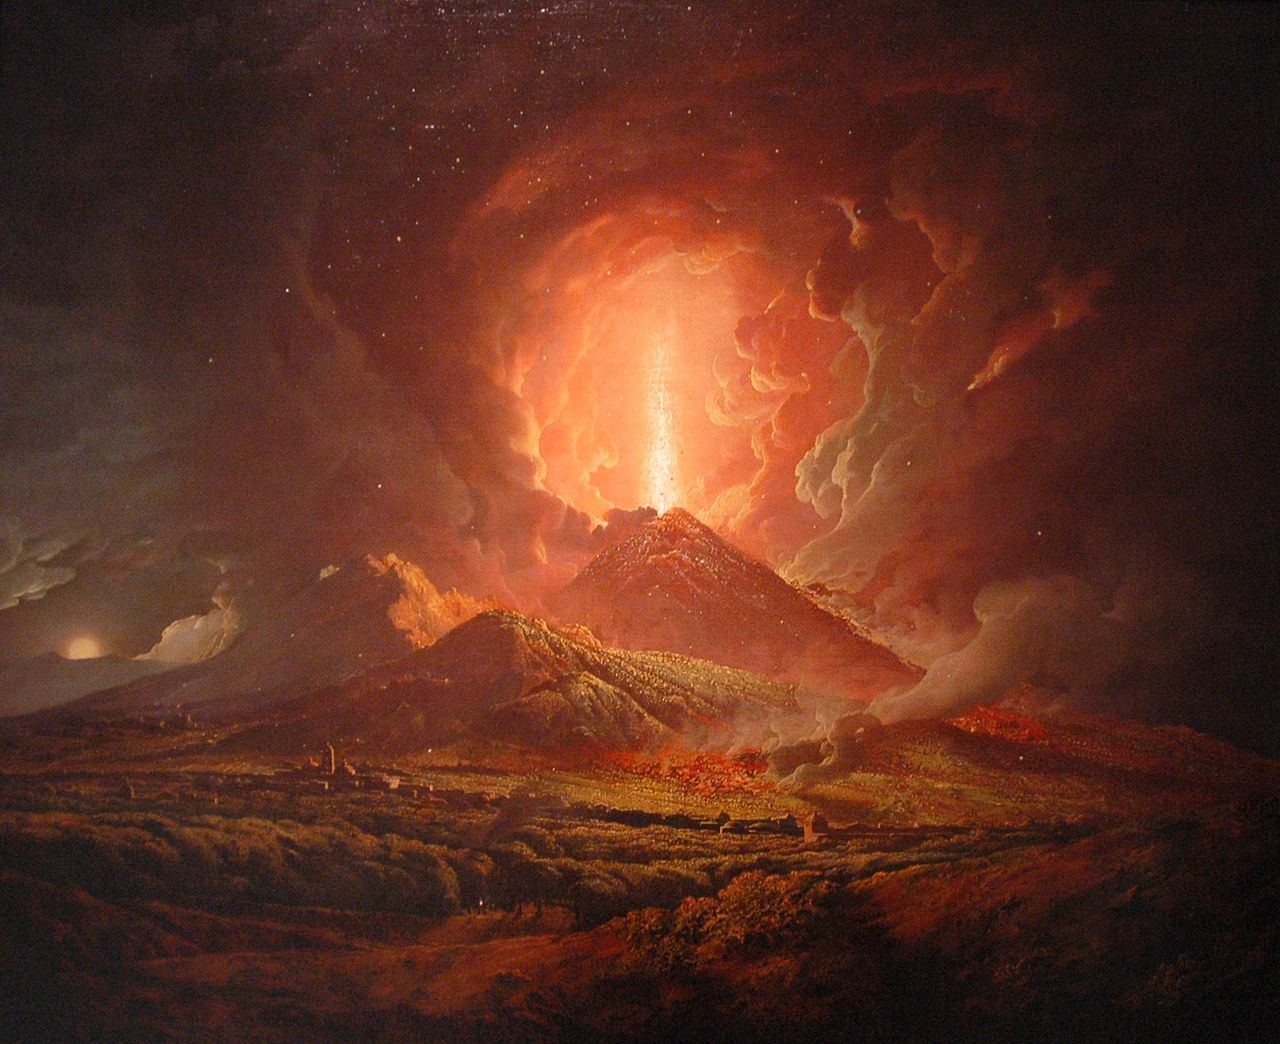
\includegraphics{figs/1280px-Joseph_Wright_of_Derby_-_Vesuvius_from_Portici.jpg}
\caption{\label{fig:unnamed-chunk-3}An eruption of Vesuvius seen from Portici, by Joseph Wright (ca. 1774-6), Dominio Publico}
\end{figure}

Sin embargo han sido los grandes episodios de contaminacion los que han gatillado su estudio y gestion por parte de los tomadores de decisiones. Entre ellos se pueden mensionar el desastre de Londres 1952 y la acidifacion de los lagos escandinavos.

\hypertarget{el-desastre-de-londres-1952}{%
\subsection{El desastre de Londres 1952}\label{el-desastre-de-londres-1952}}

{[}INSERTAR FOTO{]}

\hypertarget{acidicacion-de-los-gases-escandinavos}{%
\section{Acidicacion de los gases escandinavos}\label{acidicacion-de-los-gases-escandinavos}}

{[}INSERTAR FOTO{]}

\hypertarget{como-se-producen-las-altas-concentraciones-de-contaminantes}{%
\section{Como se producen las altas concentraciones de contaminantes}\label{como-se-producen-las-altas-concentraciones-de-contaminantes}}

\hypertarget{capa-de-mezcla}{%
\section{Capa de mezcla}\label{capa-de-mezcla}}

\hypertarget{section}{%
\section{}\label{section}}

\hypertarget{emisiones-y-sus-fuentes}{%
\section{Emisiones y sus fuentes}\label{emisiones-y-sus-fuentes}}

\hypertarget{efectos-de-la-contaminacion-atmosferica-en-la-salud}{%
\section{Efectos de la contaminacion atmosferica en la salud}\label{efectos-de-la-contaminacion-atmosferica-en-la-salud}}

\hypertarget{forzantes-climaticos}{%
\section{Forzantes climaticos}\label{forzantes-climaticos}}

\hypertarget{taller-vectores-aplicacion-de-software-de-informacion-geografica-y-modelado}{%
\chapter{Taller VECTORES: Aplicación de software de información geográfica y modelado}\label{taller-vectores-aplicacion-de-software-de-informacion-geografica-y-modelado}}

We describe our methods in this chapter.

\hypertarget{taller-raster-y-cubos-de-datos-vectoriales-aplicacion-de-software-de-informacion-geografica-y-modelado}{%
\chapter{Taller RASTER Y CUBOS DE DATOS VECTORIALES: Aplicación de software de información geográfica y modelado}\label{taller-raster-y-cubos-de-datos-vectoriales-aplicacion-de-software-de-informacion-geografica-y-modelado}}

Amanda Rehbein

Raster son informacion espaciales en una grilla espacial. Por ejemplo, vea las siguientes figuras:

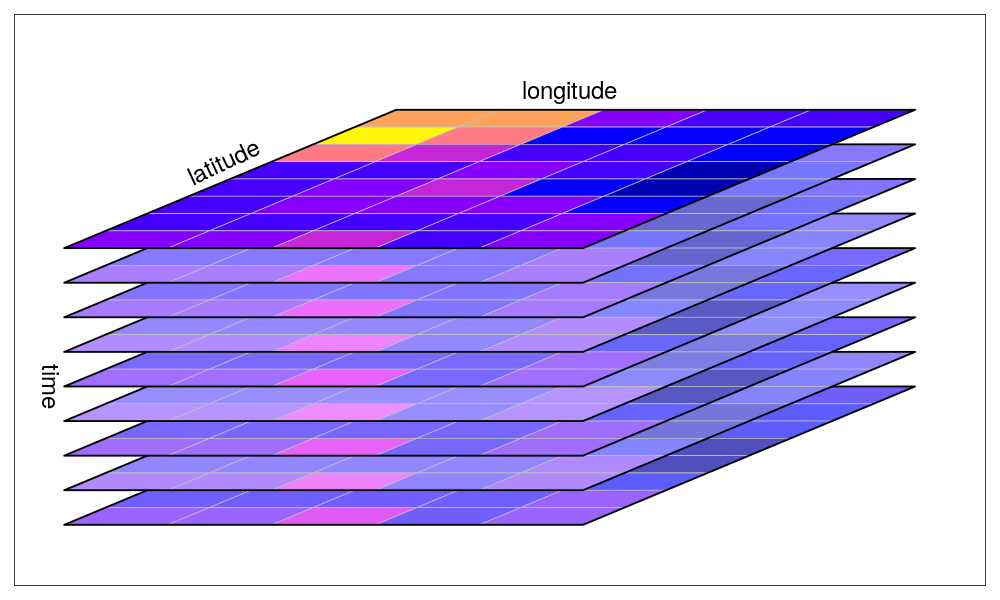
\includegraphics{figs/cube1.png}

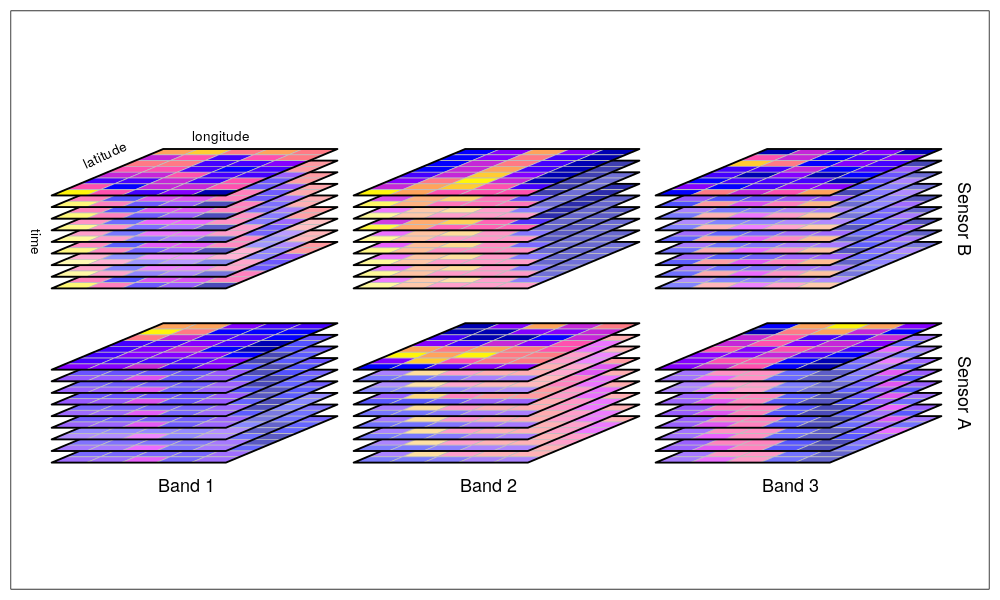
\includegraphics{figs/cube2.png}

Ejemplos con R

\hypertarget{final-words}{%
\chapter{Final Words}\label{final-words}}

We have finished a nice book.

\bibliography{book.bib,packages.bib}


\end{document}
